\documentclass[a4paper,12pt]{article}

% Font
\usepackage[T1]{fontenc}
\usepackage{gentium}

% Math packages
\usepackage{amsmath}
\usepackage{amsfonts}
\usepackage{amssymb}
\usepackage{amsthm}
\usepackage{bm}

% Define symbol shortcuts
\newcommand{\cc}{\mathcal{C}}
\newcommand{\dd}{\mathcal{D}}
\newcommand{\hh}{\mathcal{H}}
\newcommand{\xx}{{\bm x}}
\newcommand{\yy}{{\bm y}}

% Math environment
\newtheorem*{thm}{Theorem}

% Better list management:
% - vertical spacing in lists
% - items in lists start with dash not bullet point.
\usepackage{enumitem}
\setlist{label=\textemdash,
  itemsep=0pt, topsep=3pt, partopsep=0pt} 

% Include graphics
\usepackage{graphicx}
\graphicspath{ {figures/} }
\usepackage{subcaption}

% Page format 
\usepackage[top=2cm,left=2cm,right=2cm,bottom=2cm]{geometry}
\setlength{\parindent}{0pt}

\begin{document}
%%% HEADER
\raisebox{0.6in}[0in]{\makebox[\textwidth][r]{\it Unproofed version }}
\vspace{-0.7in}

\begin{center}
\bf\large MA2823: Foundations of Machine Learning \\
Chapter 4: Bayesian Learning Theory
\end{center}

\noindent
Lecturer: Chlo\'e-Agathe Azencott   
\hfill
Scribes: LOH Mathias \\
\null \hfill KIM Taehyun \\
\null \hfill MEHDI Tomas

\noindent
\rule{\textwidth}{1pt}

\medskip

%%% NOTES START HERE
\section{Introduction}
In this chapter, we aim to \textit{apply Bayes rule} for simple inference and decision problems and explain the correlation between \textit{Bayes decision rule, empirical risk minimization, maximum a priori and maximum likelihood.} In doing so, express conditional independence among random variables and finally, we aim to apply \textit{Naive Bayes algorithm}.
\section{Bayes Decision Theory}
\subsection{Probability and inference}
\textbf{Definition.}$\quad$We define a random variable $X: \Omega \rightarrow E$ an application from the set of possible outcome $\Omega$ to some set $E$. \\

Although $X$ is usually a real-valued function ($E=\mathbb{R}$), it \textit{does not} return a probability. Rather, $X$ describes some numerical property that outcomes in $\Omega$ may have - e.g, the number of heads in a random collection of coin flips. The probability that $X$ takes value $\leq 3$ is the measure of the set of outcomes $\{\omega \in \Omega : X(\omega) \leq 3\}$, denoted $P(x\leq3)$ \\ 

\textbf{Example (Coin toss).}$\quad$Let us suppose the result of tossing a coin is $x \in \{heads , tails\}$. Because this is a random process, we have \textit{incomplete information about it}. Since the result is either heads or tails, we can define this as a random variable $X$ to follow that of a \textit{Bernoulli distribution}, defined by 
\begin{equation*}
X = 
\begin{cases}
1, & \text{outcome is heads}\\
0, & \text{outcome is tails}
\end{cases}
\end{equation*}
To find the probability of obtaining $x$, we just have to find the probability $P(X=x)$ 
\subsection{Classification}
\textbf{Definition.}$\quad$ We define $C = (C_1, ..., C_k) \in \mathbb{R}^k $ the family of classes in our classification problem and a family of random variables $\xx = (X_1, ..., X_k)$ observable data which we believe is sufficient in giving us ample information about each of our classes $C_i$.\\

\textbf{Example (Credit-scoring).$\quad$} In banks, according to their past transactions, some customers are \textit{low-risk} in that they paid back their loans and the bank profited from them and other customers are \textit{high-risk} in that they defaulted. The bank would thus like to learn the class "high-risk customer"so that in the future, when there is a new application for a loan, we can check that the person obeys the class description or not and thus accept or reject the application. \\

\pagebreak
\begin{figure}[h]
\centering
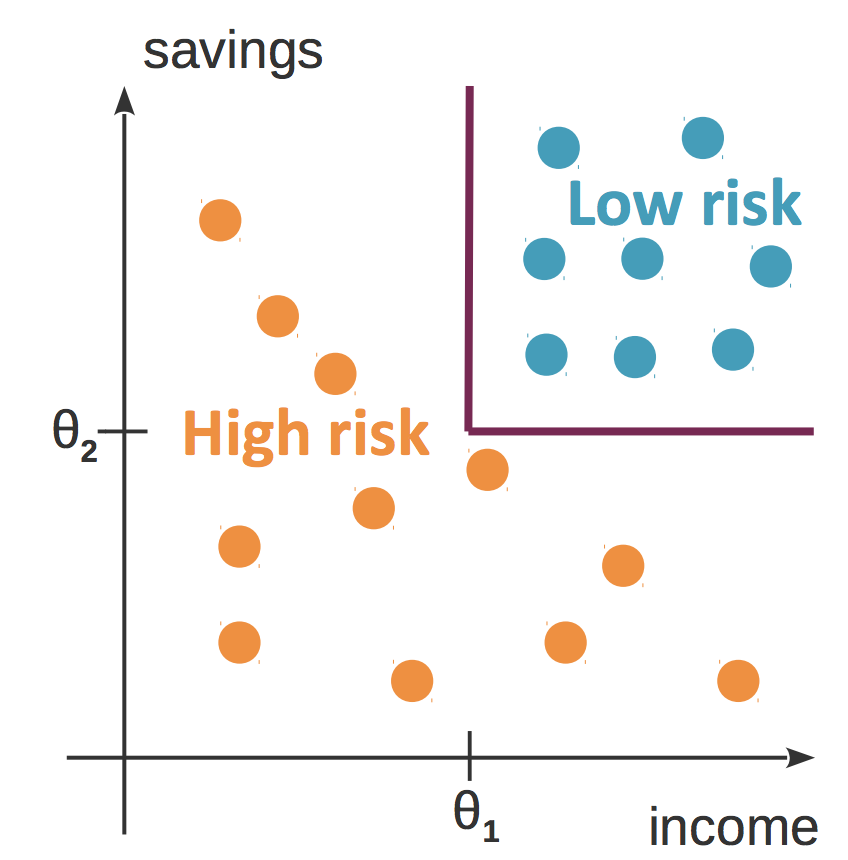
\includegraphics[scale=0.3]{creditscoring}
\caption{A classification problem with two pieces of observable information \textit{income} and \textit{savings}}
    \label{fig:creditscoring}
\end{figure}

For the simplicity of this problem, let us suppose that only two pieces of information are observable (and we observe them because we have reason to believe they give us an idea bout their credibility). These two information are \textit{income} and \textit{savings}, which we represent by two random variables $X_1$ and $X_2$. The credibility of a customer is denoted by a Bernoulli random variable $C$ conditioned on the observable $\bm{x} = [X_1, X_2]^T$ where $C=1$ indicates a high risk customer and $C=0$ indicates a low risk customer. Thus if we know $P(C|X_1, X_2)$, when a new application arrives with $X_1 = x_1$ and $X_2 = x_2$, we can
\begin{equation*}
\text{Choose}
\begin{cases}
C = 1, & \text{if } P(C=1|x_1, x_2) > 0.5 \\
C = 0, & \text{otherwise}
\end{cases}
\end{equation*}
or equivalently
\begin{equation*}
\text{Choose}
\begin{cases}
C = 1, & \text{if } P(C=1|x_1,x_2) > P(C=0|x_1,x_2)\\
C = 0, & \text{otherwise}
\end{cases}
\end{equation*}
\subsection{Decision rules}
\subsubsection{Bayes decision rule}
\begin{thm}{Bayes Theorem.}
We say the probability of obtaining a class $C$ given knowledge of $\xx$
\begin{equation*}
P(C|\bm{x}) = \frac{P(C)p(\bm{x}|C)}{p(\bm{x})}
\end{equation*}
where 
\begin{itemize}
	\item $P(C|\xx)$ defined as the \textit{posterior}
    \item $P(C)$ defined as the \textit{prior},
    \item $p(\xx|C)$ defined as the \textit{likelihood}
    \item $p(x)$ defined as the \textit{evidence}
\end{itemize}
\end{thm}
Indeed, we have in fact already seen Bayes' decision rule for a simplified case. Bringing us back to the problem of credit-scoring, the \textit{Bayes' decision rule} is simply 
\begin{equation*}
\text{Choose}
\begin{cases}
C = 1, & \text{if } P(C=1 | \xx = (x_1,x_2)) > P(C=0|\xx = (x_1,x_2))\\
C = 0, & \text{otherwise}
\end{cases}
\end{equation*}
\subsubsection{MAP decision rule}
For this decision rule, we want to pick the hypothesis that is the most probable, i.e., maximize the posterior $P(C|\xx) = \frac{P(C)p(\xx|C)}{p(\xx)}$. Again, in a 2 classifier problem, we denote $\Lambda_{\text{MAP}}(\xx) = \frac{P(C=1|\xx)}{P(C=0|\xx)}$. The MAP decision rule thus state
\begin{equation*}
\text{Choose}
\begin{cases}
C=1, & \text{if } \Lambda_{\text{MAP}}(\xx) > 1 \\
C=0, & \text{otherwise}
\end{cases}
\end{equation*}
\subsubsection{Likelihood ratio test (LRT)}
For this decision rule, we would want to test whether the likelihood ratio $\Lambda(\xx) = \frac{p(\xx|C=1)}{p(\xx|C=0)}$ is larger than or equal to ratio of priors $\frac{P(C=0)}{P(C=1)}$, i.e.
\begin{equation*}
\text{Choose}
\begin{cases}
C = 1, & \text{if } \frac{P(\xx|C=1)}{P(\xx|C=0)} > \frac{P(C=0)}{P(C=1)}\\
C = 0, & \text{otherwise}
\end{cases}
\end{equation*}

\textbf{Example (LRT with Gaussian).$\quad$}
\textit{Suppose we have $P(\xx|C=1) \sim N(4,1)$ and $P(\xx|C=0) \sim N(10,1)$ two Gaussian likelihoods with equal priors. \textbf{Derive a decision rule based on the LRT.}} \\

We first note that priors are equal, our decision rule hence becomes
\begin{equation*}
\Lambda(\xx) = \frac{p(\xx|C=1)}{p(\xx|C=0)} = \frac{e^{-(x-4)^2 /2}}{e^{-(x-10)^2 /2}} > \frac{P(C=0)}{P(C=1)} = 1
\end{equation*}
The condition that determines the decision boundary is therefore $\frac{e^{-(x-4)^2 /2}}{e^{-(x-10)^2 /2}} >1$. By taking the logarithm on the above equation, we thus obtain:
\begin{equation*}
log(\Lambda(\xx)) = 84 - 12x > 0
\end{equation*}
Which gives the decision boundary $x<7$, i.e.
\begin{equation*}
\text{Choose}
\begin{cases}
C = 1, & \text{if } x < 7\\
C = 0, & \text{otherwise}
\end{cases}
\end{equation*}
\begin{figure}[h]
\centering
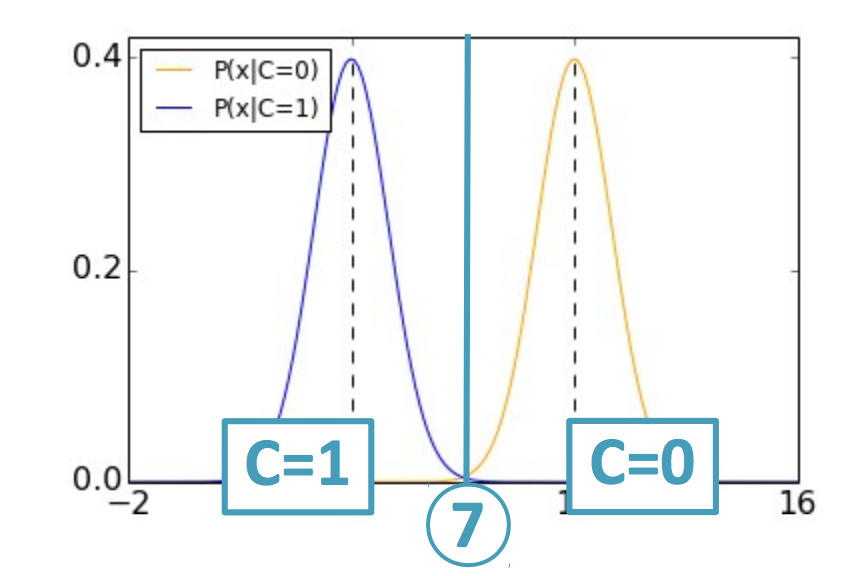
\includegraphics[scale=0.4]{lrtgaussian}
\caption{Graphical solution of the LRT with Gaussian.}
    \label{fig:creditscoring}
\end{figure}
\subsubsection{Bayes' rule for multiple classes}
In the general case, we have $K$ mutually exclusive and exhaustive classes; $C_i, i=1,...,K$. We have prior probabilities satisfying 
$$ P(C_i) \geq 0 \quad \text{and} \quad \sum\limits_{i=1}^K P(C_i)=1$$
$p(\xx|C_i)$ is the probability of seeing $\xx$ as the input when it is known to belong to class $C_i$. The posterior probability of class $C_i$ can be calculated as
$$P(C_{k}|\xx) = \dfrac{P(\xx|C_{k})P(C_{k})}{\sum\limits_{1 \leq l \leq K}{P(\xx|C_{l})P(C_{l})}}$$ and for minimum error, the \textit{Bayes' classifier} chooses the class with the highest posterior probability; that is, we
$$ \text{Choose } C_i \text{ if } P(C_i|\xx) = \max \limits_k P(C_k|\xx)$$

\subsection{Losses and risks}
It may be the case that decisions that we make are not equally good or costly. A financial firm for example, must take into account the potential gain and loss when making a decision for a loan applicant. An accepted low-risk appplicant increases profit, while a rejected high-risk applicant decreases loss. In the following sections we could consider these losses and risks and we consider that there exists $K$ different classes classes, noted $C_{i}, i = 1,...,K$. 

\subsubsection{Penalization}
\textbf{Definition. $\quad$} Let us define action $\alpha_i$ as the decision to assign the input to class $C_i$ and $\lambda_{kl}$ as the \textit{quantity of loss} for taking action $\alpha_k$ when the input actually belongs to $C_l$. The \textit{expected risk} is the sum of the risks for all the classes that the point could belong to times the probability that it belongs to the given class, that is,

\begin{equation*}
R(\alpha_k|\xx) = \sum_{l = 1}^{K}{\lambda_{kl}P(C_l|\xx)}
\end{equation*}

We note that this becomes the case of choosing the \textit{actions with minimal risks}, i.e., we choose $\alpha_i$ if  $R(\alpha_i|\xx) = \min\limits_k R(\alpha_k|\xx)$ or alternatively
\begin{equation*}
R(\alpha_k|\xx) = \arg \min\limits_ R(\alpha_k|\xx)
\end{equation*}


\subsubsection{0/1 Loss}
\textbf{Definition. $\quad$}Let us define $K$ actions $\alpha_i, i=1,...,K$. In the special case of the 0/1 \textit{loss case} where
\begin{equation*}
\lambda_{kl} =
\begin{cases}
0, & \text{if } k = l\\
1, & \text{if } k \neq l
\end{cases}
\end{equation*}
\textit{where all correct decisions have no loss and all errors are equally costly.} The risk of taking action $\alpha_i$ is
$$ R(\alpha_i|\xx) = 1 - P(C_i|x)$$
Thus to minimize risk, we choose the most probable class. Note that this is a \textit{special case} and rarely do applications have a symmetric 0/1 loss. This however serves as a simple model for analysis in this course!

\subsubsection{Reject}
In some applications, wrong decisions may have very high cost, and it is generally required that a more complex (e.g, manual classification) be made if automation dictates a \textit{low certainty of its decision}. We thus create an additional \textit{action of reject} $\alpha_{K+1}$ which is the option to not take any decision. A possible loss function is thus (following the example of 0/1 loss),
\begin{equation*}
\lambda_{kl} = 
\begin{cases}
\lambda \text{ if } k = K+1
\\
0 \text{ if } k = l
\\
1 \text{ otherwise}
\end{cases}
\end{equation*} 
The decision is therefore taken according to:
\begin{equation*}
\begin{cases}
\text{Choose } C_l, & \text{if } R(\alpha_l|\xx) < R(\alpha_k|\xx)\, \forall k \neq l \textbf{ and } R(\alpha_l|\xx) < R(\alpha_{K+1}|\xx) \\
\text{reject } & \text{otherwise}
\end{cases}
\end{equation*}

We choose $0 \leq \lambda \leq 1$, otherwise $\lambda = 0$ will always reject whereas $\lambda = 1$ will never reject!
\subsubsection{Bayes Risk}
We have thus far seen the different ways we could construct the risks of our problems. In this section, we introduce the notion of the total expected risk that we should expect in a classification problem. \\

\textbf{Definition. $\quad$}We call \textbf{Bayes' risk} the overall expected risk, the sum of all risks of taking any action $\alpha_k$:
\begin{equation*}
R(\xx) = \sum_{k=1}^{K} R(\alpha_k|\xx) = \sum_{k=1}^{K}{\sum_{l = 1}^{K}{\lambda_{kl}P(C_{l}|\xx)}}
\end{equation*}

\subsubsection{Discriminant functions}
\textbf{Definition. $\quad$}Classification can also be seen as implementing a set of \textit{discriminating functions}, \linebreak $f_i(\xx), i = 1,...,k$, such that we choose $C_i$ if $f_i(\xx) = \max_k f_k(\xx)$. We represent the Bayes' classifier by setting:
\begin{equation*}
f_{k}(\xx) = - R(\alpha_k| \xx)
\end{equation*}
Furthermore, we can define these discriminant functions into $K$ \textit{decision regions} $\mathcal{R}_1,...,\mathcal{R}_K$, which separated by \textit{decision boundaries} which separates one class from another. These decision regions are given by 
$$R_{k} = \{ x : f_{k}(\xx) = \max\limits_{l}f_{l}(\xx) \}$$ 
\begin{figure}[h]
\centering
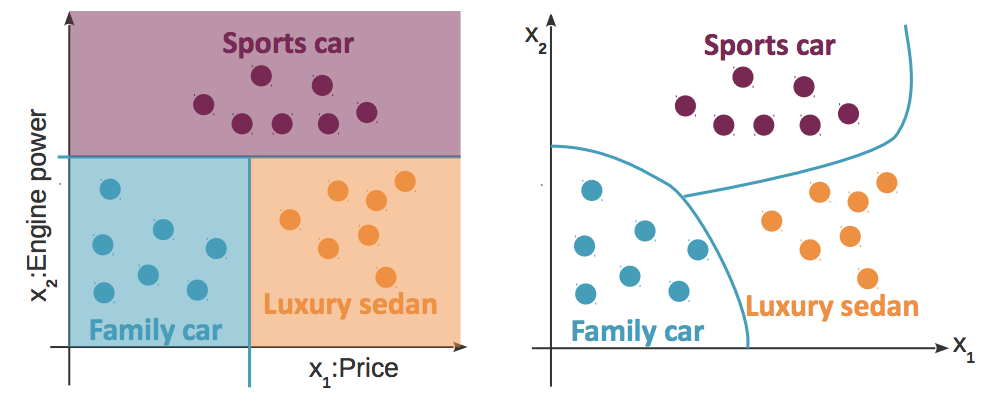
\includegraphics[scale=0.25]{boundaries}
\caption{Example of 3 decision boundaries}
    \label{fig:creditscoring}
\end{figure}
\subsubsection{Supplement: losses for regression}
We introduce the following losses commonly seen and used in regression
\begin{itemize}
\item \textbf{Square loss}: $L(f(\xx),y) = (f(\xx) - y)^{2}$. \\This loss functions has the problem of penalizing heavily outliers, which results in increasing the numerical error with unclean data. The two next loss functions seek to solve that problem.
\item $\bm{\epsilon}$ - \textbf{insensitive loss}: $L(f(\xx),y) = (|f(\xx) - y| - \epsilon)_{+}$

\item \textbf{Huber Loss:}
$
L_{\delta}(f(\xx),y) = \begin{cases}
\dfrac{1}{2}(y-f(\xx))^{2},& \text{ if } | y - f(\xx) | \leq \delta
\\
\delta |y - f(\xx)| - \delta^{2}/2,& \text{otherwise}
\end{cases}$ \\ 
However, these two functions are not smooth, which can cause problems in algorithms which seek to minimize them. 
\end{itemize}
\begin{figure}[h]
\centering
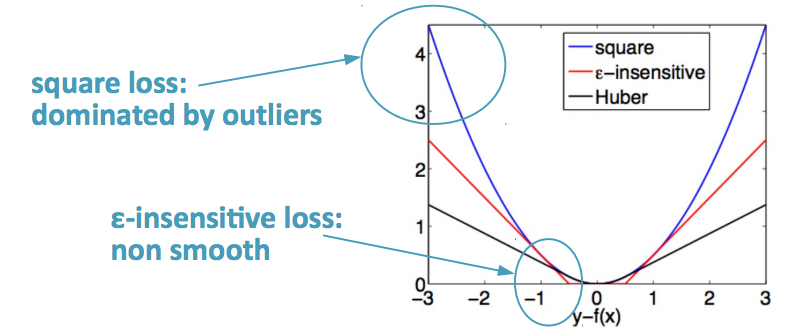
\includegraphics[scale=0.3]{errorsummary}
\caption{Summary of regression errors}
    \label{fig:creditscoring}
\end{figure}
\subsection{Empirical risk minimization}
The main idea is that the loss function $L(f(\xx),y)$ is small when $f(\xx)$ predicts y well. We have
\begin{itemize}
\item Expected risk: $R = \mathbb{E} [ L(f(\xx),y) ]$
\item Empirical risk: $R_n = \frac{1}{n} \sum_{i=1}^{n} L(f(\xx^i),y^i)$
\item ERM estimator of the functional class F is the solution, when it exists, of
$\hat{f}_n = \arg \min\limits_{f \in \mathcal{F}} R_n(f)$
\end{itemize}
However ERM is ill posed and it can be that an infinite number of solutions minimize the empirical risk to zero. ERM is also not statistically consistent. Law of large numbers is only true if capacity (VC-dimension) of $f$ is not too large.
\begin{figure}[h]
\centering
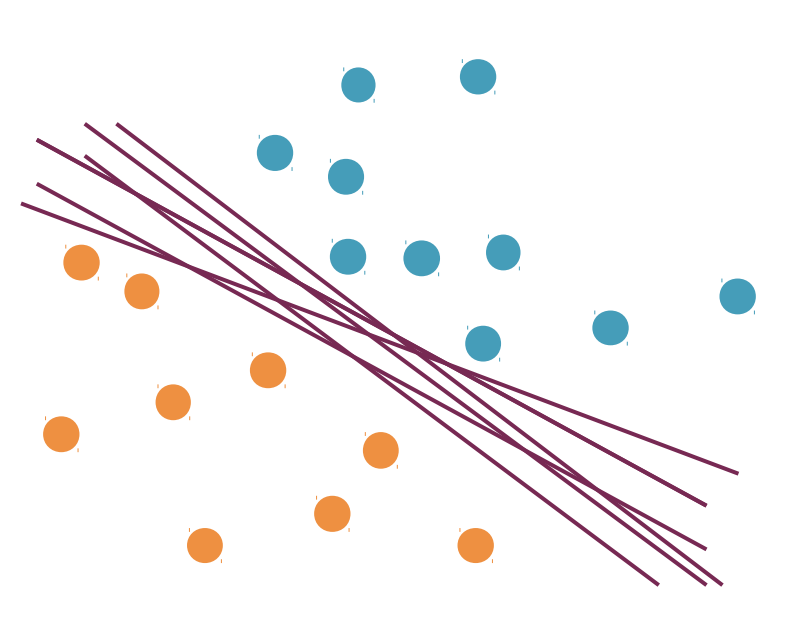
\includegraphics[scale=0.3]{erminfinite}
\caption{Ill posed problem: infinite solutions!}
    \label{fig:creditscoring}
\end{figure}
\section{Multivariate classification: Naive Bayes}
\subsection{Naive Bayes}
Naive Bayes is a \textit{multivariate classification}, which is to say, $\xx$ is multidimensional. We also have an assumption that the variables $\xx = (x_1, x_2,...,x_p)$ are conditionally independent, i.e.,
$$p(x_i|C_k,x_j) = p(x_i|C_k)$$
By applying this property to Bayes' rule that we have seen previously,
\begin{align*}
P(C_k|\xx) &= \frac{p(\xx|C_k)P(C_k)}{\sum_{k=1}^{K}p(\xx|C_k)P(C_k)} \\
		   &= \frac{P(C_k)p(x_1|C_k)p(x_2|C_k)\cdot \cdot \cdot p(x_p|C_k)}{\sum_{k=1}^{K}p(\xx|C_k)P(C_k)}\\
           &= \frac{1}{Z}P(C_k)p(x_1|C_k)p(x_2|C_k)\cdot \cdot \cdot p(x_p|C_k)
\end{align*}
Where we note $\frac{1}{Z}$ a scaling factor independent of $C_k$. 
\subsection{Algorithms}
\subsubsection{Maximum a posteriori (MAP) estimation}
We recall in a \textit{MAP decision rule}, we pick the hypothesis that is most probable (Homework 3!). For Naive Bayes, the \textit{MAP decision rule} is defined by
\begin{align*}
\hat{y} = \arg \max\limits_{k=1,..,K}p(C_k) \Pi_{i=1}^n p(\xx^i|C_k) 
\end{align*}
\subsubsection{Bernoulli Naive Bayes}
In the case of a \textit{binary classification problem} (2 classes), we can define each sample as the outcome of $p$ Bernoulli trials, with the assumption that each trials are \textit{independent} from the others. Then the decision rule for Bernoulli Naive Bayes is based on
$$p(x_j|C_k) = p_j^{x_j}(1-p_j)^{(1-x_j)}$$
\subsubsection{Gaussian Naive Bayes}
We further assume that $p(x_j|C_k)$ is a \textit{univariate Gaussian} and the decision rule is defined as
$$p(x_j|C_k) = \frac{1}{\sigma \sqrt{2\pi}}e^{-(x-\mu)^2/(2\sigma^2)}$$ 
where $\mu$ and $\sigma$ are estimated using maximum likelihood.
\begin{figure}[h]
\centering
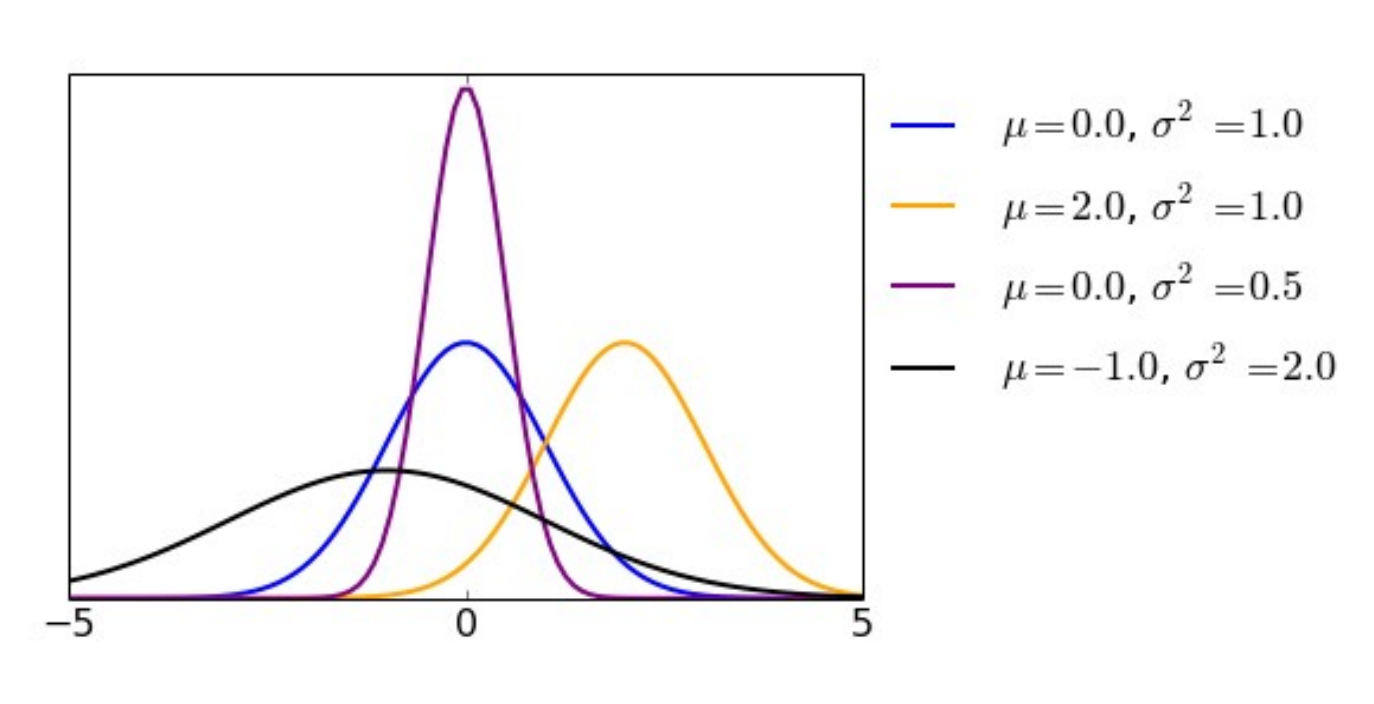
\includegraphics[scale=0.3]{naivegaussian}
\caption{Naive Gaussian examples with varying $\mu$ and $\sigma$}
    \label{fig:creditscoring}
\end{figure} \pagebreak
\subsection{Bayesian model selection}
The key idea of this section is that we can also take priors on models, and we denote it as $p$(model). Similar to previous sections, we can thus define a decision rule
\begin{equation*}
p(\text{model}|\text{data}) = \frac{p(\text{data}|\text{model})p(\text{model})}{p(\text{data})}
\end{equation*}
In addition, if we take the log on both sides of the equation, we obtain,
$$\log p(\text{model}|\text{data}) = \log p(\text{data}|\text{model}) + \log p(\text{model}) - \log {p(\text{data})}$$
where we can further define $\log p(\text{data}|\text{model})$ as the \textit{training error} and $\log p(\text{model})$ the \textit{complexity} of our model. We can also take the maximum a posteriori (MAP) which is similar to minimizing 
$$E' = \text{empirical error } + \bm{\lambda} \text{ model complexity}$$
\end{document}


